%%%%%%%%%%%%%%%%%%%%%%%%%%%%%%%%%%%%%%%%%%%%%%%%%%%%%%%%%%%%%%%%%%%%%%%%%%%%%%
%
% PROJECT PROPOSAL  DESCRIPTION:
%   A concise description of the main concepts of the proposed project.
%
% RESEARCH:
%   A list of research activities which led to this project.
%
% EXPERIMENTS:
%   A list of the experiments performed which supported the research.
%
%%%%%%%%%%%%%%%%%%%%%%%%%%%%%%%%%%%%%%%%%%%%%%%%%%%%%%%%%%%%%%%%%%%%%%%%%%%%%%%
% Define a single space environment (copied from doublespace.sty)
% e.g. \begin{singlespace}
%         single-spaced text
%      \end{singlespace}

\documentclass[12pt,american]{article}
\usepackage{fullpage}
\usepackage{bbm}
\usepackage{url}
\usepackage{subfigure}
\usepackage{babel}
\usepackage{times}
\usepackage{graphicx}
\usepackage{amssymb}
\usepackage{lscape}
\usepackage{verbatim}
\usepackage{enumerate}
\usepackage{afterpage}
\usepackage{setspace}


\begin{document}
\thispagestyle{empty} 
\begin{center}
{\em MS Project Proposal}\\
\vspace{.5in}
{\large \bf An Aspect Oriented Programming Framework for C\#}\\
\vspace{.5in}
{\bf Wei Liao}\\
\vfill
\
{\em Committee Chair:} Prof. James E. Heliotis\\
\vspace{0.1in}
{\em Reader: } Prof. Fereydoun Kazemian\\
 \vspace{0.1in}
{\em Observer: } Prof. Matthew Fluet\\
 \vspace{0.1in}
Department of Computer Science\\
B. Thomas Golisano College of Computing and Information Sciences \\
Rochester Institute of Technology \\
Rochester, New York \\ [0.3in]
\vspace{0.5in}
\today{}\\
\end{center}
\vfill

%%%%%%%%%%%%%%%%%%%%%%%%%%%%%%%%%%%%%%%%%%%%%%%%%%%%%%%%%%%%%%%%%%%%%%%%%%%%%%%
%%  Collection of useful abbreviations.
\newcommand{\etc} {\emph{etc.\/}}
\newcommand{\etal}{\emph{et~al.\/}}
\newcommand{\eg}  {\emph{e.g.\/}}
\newcommand{\ie}  {\emph{i.e.\/}}
%%%%%%%%%%%%%%%%%%%%%%%%%%%%%%%%%%%%%%%%%%%%%%%%%%%%%%%%%%%%%%%%%%%%%%%%%%%%%%%


%%%%%%%%%%%%%%%%%%%%%%%%%%%%%%%%%%%%%%%%%%%%%%%%%%%%%%%%%%%%%%%%%%%%%%%%%%%%%%%
% Abstract
\section*{Abstract}
Aspect Oriented Programming (AOP) is a paradigm that let programmers isolate and separate cross-cutting concerns from the basis of their program. The concept is relatively new, so very few languages has native support for this capability, support in toolings such as IDE integration is also rare. In this project we will design and implement a framework that provides AOP functionality for C\# via IL code weaving and integrate it with the Visual Studio IDE.
%%%%%%%%%%%%%%%%%%%%%%%%%%%%%%%%%%%%%%%%%%%%%%%%%%%%%%%%%%%%%%%%%%%%%%%%%%%%%%%
\vfill{}

%%%%%%%%%%%%%%%%%%%%%%%%%%%%%%%%%%%%%%%%%%%%%%%%%%%%%%%%%%%%%%%%%%%%%%%%%%%%%%%
% This is where the main body of the capstone proposal starts
\setcounter{page}{0} 
\newpage{}

\section{Introduction}
This part of the proposal should be a couple of paragraphs that
describe the reason for your proposal and your project/thesis area at
high level.

\section{Background}
Procedural Language such as C achieves modularity by grouping codes into subroutines or functions, whereas Object Oriented Programming (OOP) such as JAVA or C\# go one step further, and they allow programmers to abstract real world object into properties and behaviors.

While both paradigms give programmers of that languages the ability to make their code cleaner and more reusable, they are not sufficient to clearly capture some of the important software design decision [1].

In OOP languages, while various objects corresponding to the real world or business requirement can be developed, the usage of the instances of all those objects could still be scattered throughout different modules of the program. Overtime, these tangled cross-cutting concerns [1] can be difficult and expensive maintenance. One of the often cited example of such concern is exception handling, the ability to for programs to handle errors or die gracefully.

To handle exception in our code, in its most basic form we can have the follow try..catch block:
\begin{verbatim}
public void SomeFunction() {
    try {
		//this will fail
		var result = 1 / zero;
    } catch (Exception e) {
		//log exception to file, etc
        Utility.LogToFile(e);
    }
}
\end{verbatim}

Now imagine if you have 10,000 functions in your program that can potentially throw errors, you would have to apply the try..catch block on all of them. And since your program most likely will consist of many modules, it will mean this repetitive pattern will cut through and appears in all your modules.

Imagine again, what if you need to fine tune this try..catch block to catch a specific exception so your program can act accordingly, or instead of logging to a file you want to log it to a database. In the worst case you would have to make the change to all 10,000 of your functions.

The problem is how to isolate those cross-cutting concerns from loitering your program. Aspect Oriented Programming technique [1] can be used to cleanly separate such concerns.

\section{Related Work}
Describe what work others have already done in this area. You do need
several citations, and this is how you cite a book by
Silberschatz~\cite{Silberschatz05-text} or a paper by
Dumont~\cite{Dumont2007-robots}.

\section{Hypothesis}
Summarize what you think the problem is, and what your hypothesis
is. Here is a small example based on a successful project by Priyanka
Sinha: ''Using one technique for schema matching does not seem
adequate. The hypothesis underlying this sproject is that a holistic
approach to schema matching based on the three techniques described
earlier would do an effective approach to schema matching.''

Additional description to circumscribe the work so that the reader
knows what you plan to do to establish your hypothesis.

\section{Approach and Methodology}
\subsection{Architecture Overview}
There are many approaches on how to implement an AOP framework. The approach I plan to take is to perform post compilation weaving. Figure 1 shows an overview of how the AOP framework will fit in the overall C\# compilation process.

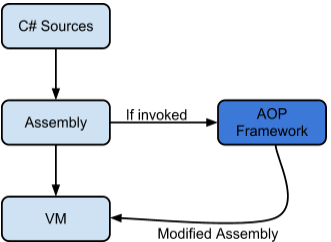
\includegraphics[width=331px,keepaspectratio=true]{model_overview.png}

Describe how you plan to design and implement a solution. 

You must also describe how you would use your solution to establish the validity of your hypothesis. Explain the measurements you plan to conduct and how these would establish the validity (or invalidity) of your hypothesis.

\subsection{Compile Time Weaving}
Within this method there are a few variants of compile time weaving, one is to preprocess the source files, to perform text transformation to weave all the aspects at the right locations of the source, then just let the compiler take over and compile as normal.

The other type is MSIL rewriting, as indicated by figure 1 , the C\# compiler performs a compile on the source files to generate the assembly. This assembly is then fed into the AOP Framework, which will proceed to rewrite the MSIL instruction calls to weave in the aspects.

There are obvious advantages and disadvantages to each method. [Give some examples of what those are?]

\subsection{Platform, Languages and Tools}
This project will be developed using C\#, on the Windows 7 using Visual Studio 2010. When performing IL rewriting there are a few options available, one is to use the Reflection.Emit library that comes with the .NET Framework, however all my researches points to that this library represents only a subset of the MSIL instructions, the missing instruction might prove to be a problem later on.

Another option is to use the Profiler API by Microsoft, however this API is intended as a debugging feature, and therefore is unsuitable to be used in production environment.

While I can opt to invest my time on learning and rolling my own IL rewriter, a more practical option is probably to use a 3rd party library. Mono is an open source implementation of the C\# compiler, Cecil is a project within the Mono project that provides IL rewriting. Preliminary evaluation of the tool seems to be pretty feature complete and flexible enough to allow me to do what I need to do. However documentation for Cecil is next to non-existent, it works with low level MSIL, so I expect the learning curve is probably deep.

The following utility tools will also be heavily used during development: ILSpy, ILDASM and PEVerify. ILSpy is an open source application that dis-assemble assembly to show IL instructions. ILDASM does the same but comes from Microsoft’s .NET Framework. PEVerify is a Microsoft Window SDK tool, it will be used to ensure that the modified assembly produced is a correct assembly.

\section{Roadmap}

Here you need to describe your project plan, with dates and deliverables. 

You must review the CS graduate handbook for details, and yes, make
sure you also address all of the handbook's requirements for a
proposal.

The following table shows my tentative schedule for the major phases of the project.

\begin{table}[h]
\centering
\begin{tabular}{|l|l|l|}
\hline
Date & Action & Status\\
\hline
07/07/2012 & Pre-Proposal & Accepted\\
07/09/2012 & Proposal & In-progress\\
07/20/2012 & Begin development of the framework & In-progress\\
08/20/2012 & Finish development & Started\\
- & Testing and analysis & - \\
- & Finish report & - \\
- & Defense & - \\
\hline
\end{tabular}
\caption{Timeline}
\label{tab:template}
\end{table}

%%%%%%%%%%%%%%%%%%%%%%%%%%%%%%%%%%%%%%%%%%%%%%%%%%%%%%%%%%%%%%%%%%%%%%%%%%%%%%%

%%%%%%%%%%%%%%%%%%%%%%%%%%%%%%%%%%%%%%%%%%%%%%%%%%%%%%%%%%%%%%%%%%%%%%%%%%%%%%%
\bibliographystyle{plain}
% Single space the bibliography to save space.
\singlespacing
\bibliography{Proposal}
%%%%%%%%%%%%%%%%%%%%%%%%%%%%%%%%%%%%%%%%%%%%%%%%%%%%%%%%%%%%%%%%%%%%%%%%%%%%%%%


\end{document}
